  \documentclass[12pt]{exam}
\usepackage{amsthm}
\usepackage{libertine}
\usepackage[utf8]{inputenc}
\usepackage[margin=1in]{geometry}
\usepackage{amsmath,amssymb}
\usepackage{multicol}
\usepackage[shortlabels]{enumitem}
\usepackage{siunitx}
\usepackage{cancel}
\usepackage{graphicx}
\usepackage{float}
\usepackage{pgfplots}
\usepackage{algpseudocode}
\usepackage{listings}
\usepackage{tikz}


\pgfplotsset{width=10cm,compat=1.9} \usepgfplotslibrary{external}
\tikzexternalize

\newcommand{\class}{Grafos} % This is the name of the course 
\newcommand{\examnum}{Tarea 1} % This is the name of the assignment
\newcommand{\examdate}{\today} % This is the due date
\newcommand{\timelimit}{}





\begin{document}
\pagestyle{plain}
\thispagestyle{empty}

\noindent
\begin{tabular*}{\textwidth}{l @{\extracolsep{\fill}} r @{\extracolsep{6pt}} l}
	\textbf{\class} & \textbf{Name:} & \textit{Sergio Montoya}\\ %Your name here instead, obviously 
	\textbf{\examnum} &&\\
	\textbf{\examdate} &&
\end{tabular*}\\
\rule[2ex]{\textwidth}{2pt}
% ---

\begin{enumerate}
  \item La figura $1.6$ del libro ilustra un grafo autocomplementario, el pentagono, que tiene cinco vertices. Encuentre otro grafo autocomplementario con cinco vertices. No basta con dar el dibujo. Explique por que su grafo si es autocomplementario y explique por que no es isomorfo al pentagono.

En este caso podemos tener el grafo:
\begin{figure}[H]
  \centering
  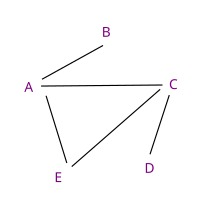
\includegraphics[width=0.3\textwidth]{Graficas/Grafo1.jpeg}
  \caption{Grafo autocomplementario.}
  \label{fig:Graficas-Grafo1-jpeg}
\end{figure}

Que en este caso su grafo complementario seria:

\begin{figure}[H]
  \centering
  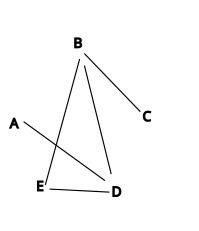
\includegraphics[width=0.3\textwidth]{Graficas/Grafo2.jpeg}
  \caption{Complemento del grafo \ref{fig:Graficas-Grafo1-jpeg}}
  \label{fig:Graficas-Grafo2-jpeg}
\end{figure}

Y podemos hacer una transformación del siguiente estilo para que quede:

\begin{figure}[H]
  \centering
  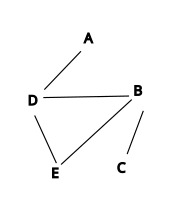
\includegraphics[width=0.3\textwidth]{Graficas/Grafo3.jpeg}
  \caption{Transformación del grafo \ref{fig:Graficas-Grafo2-jpeg} para que quede como el grafo \ref{fig:Graficas-Grafo1-jpeg}}
  \label{fig:Graficas-Grafo3-jpeg}
\end{figure}

Ademas, sabemos que es imposible que sea isomorfa a el pentagono dado que solo hay un vertice con $2$ arcos y el pentagono tiene todos sus vertices con este numero de arcos.

  \item Suponga que $G$ tiene una lista de grados $D=\left( d_1,\ldots,d_n \right) $. ¿Cual es la lista de grados del grafo complemento $\overline{G}$? Explique su respuesta.

    En este caso recordemos que $\overline{G}$ es la dupla $\overline{G}=\left( \overline{V},\overline{E} \right) $ donde $\overline{V}=V$ y $\overline{E}=\begin{pmatrix} n\\2 \end{pmatrix}\backslash E $ por lo tanto, todos los arcos que \textit{Faltan} en $G$ estaran en $\overline{G}$ y como el maximo de arcos para cada nodo es $n-1$ entonces manteniendo el mismo orden la lista quedaria: \[
    \overline{D}=\left( n-1-d_1,\ldots,n-1-d_n \right) 
    .\] 



  \item Use el algoritmo GraphGen visto en clase para construir un grafo con la lista de grados \[
  \left( 3,3,3,3,3,3 \right) 
  .\] o para determinar que la lista no es grafica. Su respuesta debe consistir de una tabla como las que se usaron en clase indicando como se va reduciendo la lista de grados, la matriz de adyacencia que se tiene al salir del algoritmo (tambien como se hizo en el ejemplo en clase) y decir explicitamente si la lista resulto ser grafica o no.

  \textbf{Tabla de Reducción de la Lista:}

  \begin{table}[H]
    \centering
    \caption{Tabla de reducción de la lista de la lista grafica $\left( 3,3,3,3 \right) $}
    \label{tab:list1}
    \begin{tabular}{|c|c|c|c|}
      \hline
    3 & 3 & 3 & 3 \\
    0 & 2 & 2 & 2 \\
    0 & 0 & 1 & 1 \\
    0 & 0 & 0 & 0 \\
    \hline
    \end{tabular}
  \end{table}

  \textbf{Matriz de Adyacencia:}

  \begin{align*}
    \begin{pmatrix} 0 & 1 & 1 & 1 \\
      1 & 0 & 1 & 1 \\
      1 & 1 & 0 & 1 \\
      1 & 1 & 1 & 0
    \end{pmatrix} 
  .\end{align*}

  \textbf{¿La lista es Grafica?: } Si

  \item Use el algoritmo GraphGen visto en clase para construir un grafo con la lista de grados \[
  \left( 7,6,6,6,5,5,2,1 \right) 
  .\]
  o para determinar que la lista no es grafica. Su respuesta debe consistir de una tabla como las que se usaron en clase indicando como se va reduciendo la lista de grados, la lista de adyacencia que se tiene al salir del algoritmo (tambien como se hizo en el ejemplo en clase) y decir explicitamente si la lista resulto ser grafica o no.


  \textbf{Tabla de Reducción de la Lista:}

  \begin{table}[H]
    \centering
    \caption{Tabla de reducción de la lista de la lista grafica $\left( 7,6,6,6,5,5,2,1 \right) $}
    \label{tab:list1}
    \begin{tabular}{|c|c|c|c|c|c|c|c|}
      \hline
      7 & 6 & 6 & 6 & 5 & 5 & 2 & 1 \\
      0 & 5 & 5 & 5 & 4 & 3 & 1 & 0 \\
      0 & 0 & 4 & 4 & 3 & 2 & 0 & 0 \\
      0 & 0 & 0 & 4 & 3 & 1 & -1 & 0\\
    \hline
    \end{tabular}
  \end{table}

  \textbf{Lista de Adyacencia:}
  \begin{table}[H]
    \centering
    \caption{Lista de adyacencia para la lista $\left( 7,6,6,6,5,5,2,1 \right) $}
    \label{tab:listaadj}
    \begin{tabular}{|c|c|}
      \hline
     $u_1$& $u_2,u_3,u_4,u_5,u_6,u_7$ \\
     $u_2$ & $u_3, u_4, u_5, u_6$\\
     $u_3$ & Fallo \\
     $u_4$ & Fallo \\
     $u_5$ & Fallo \\
     $u_6$ & Fallo \\
     $u_7$ & Fallo \\
     \hline
    \end{tabular}
  \end{table}

  \textbf{¿La lista es Grafica?: } No

\item Sea $G$ un grafo simple con $n$ vertices y representado por medio de una matriz de adyacencia $Adj$. Escriba un algoritmo (en pseudocodigo) que calcule el número de vertices del grafo que tienen grado impar. ¿Cual es la complejidad de su algoritmo? (Use notación $O\left( f\left( n \right)  \right) $ para su respuesta).

  
  \begin{algorithmic}[1]
    \Procedure{ContarNodosImpares}{$Adj$}
    \State $Even \gets 0$
    \For{  $u\gets 1$ to $n$ }
    \State $Edges \gets 0$
    \For{ $v\gets 1$ to  $n$}
    \If{$Adj\left[ u,v \right] = 1$}
    \State $Edges \gets Edges + 1$
    \EndIf
    \EndFor
    \If{ $Edges\equiv_21$}
    \State  $Even \gets Even+1$
    \EndIf
    \EndFor
    \EndProcedure
  \end{algorithmic}

  En este caso tenemos que analizar por partes. En particular, debemos considerar tres partes relevantes:
  \begin{enumerate}
    \item Fuera de los \textbf{for} hay 1 instrucción
    \item En el primer \textbf{for} hay 5 instrucciones tres asignaciones de variable, una suma y una comparación.
    \item En el segundo \textbf{for} hay 4 instrucciones 2 asignaciones de variable, una suma y una comparación.
  \end{enumerate}

  Entonces tenemos que sumar todas estas instrucciones
  \begin{align*}
    1 + \sum_{i=1}^{n} \left(5 + \sum_{j=1}^{n} 4\right)\\
    1 + \sum_{i=1}^{n} 5 + \sum_{i=1}^{n} \sum_{j=1}^{n} 4\\
    1 + 5n + \sum_{i=1}^{n} 4n\\
    1 + 5n + 4n^2
  .\end{align*}
  
  ahora bien, sabemos que $1<n^2$ y que $5n<5n^2$ por lo tanto para encontrar $O\left( f\left( n \right)  \right) $ vamos a utilizar esto de la siguiente manera:
  \begin{align*}
    1 + 5n + 4n^2 < n^2 + 5n^2 + 4n^2\\
    n^2 + 5n^2 + 4n^2\\
    n^2\left( 1 + 5 + 4 \right) \\
    10n^2
  .\end{align*}
  
  Por lo tanto este algoritmo es $O\left( n^2  \right) $ donde $c$ es $10$ y $N$ es $1$

\item Demuestre que si  $G$ es un grafo simple con $n$ vertices y $\epsilon$ arcos, entonces $\log\left( \epsilon \right) = O\left( \log\left( n \right)  \right) $

  En este caso iniciamos por notar que el maximo valor de $\epsilon$ que puede tomar es $\left( n-1 \right) n$ en el caso de el grafo completo. Por lo tanto, si logramos mostrar que $\log\left( n \left( n-1 \right)  \right) = O\left( n^2 \right) $ entonces sabremos que para cualquier otro $\epsilon$ esto se cumple pues a de ser menor. Por lo tanto:
  \begin{align*}
    \log\left( n\left( n-1 \right)  \right) = \log\left( n \right) + \log\left( n-1 \right) 
  .\end{align*}

  Ahora bien note que $n\le n^2$ siempre que $n\in \mathbb{N}$ que dado que hablamos de los vertices de un grafo podemos asumir esto como cierto. Por lo tanto
  \begin{align*}
    \log\left( n \right) + \log\left( n-1 \right) \le \log\left( n^2 \right) + \log\left( n^2 \right) \\
    \le 2\log\left( n^2 \right) 
  .\end{align*}

  Hay un caso en el que no funcióna y es con el $0$ dado que cuando $n=0$ se da que $\epsilon = 0$ pero en ese caso los dos estan indefinidos.

\item Sean $a,b$ enteros positivos. Demuestre que $f\left( n \right) = n^a$ es $O\left( n^{b} \right) $ si y solo si $a\le b$.
  \begin{enumerate}
    \item $"\Rightarrow"$

      Asuma que $n^{a}=O\left( n^{b} \right) $ entonces sabemos que
      \begin{align*}
        0\le n^{a} \le c\cdot n^{b}
      .\end{align*}
      
      Siempre que $n\ge N$ donde $N,c \in \mathbb{Z}^{+}$. Ahora bien, dado que $n^{a}=O\left( n^{b} \right) $ sabemos que 
      \begin{equation*}
      \displaystyle \lim_{n\to \infty}\frac{n^{a}}{n^{b}}
    \end{equation*}
       existe. Por lo tanto
      \begin{align*}
        \lim_{n \to \infty} \frac{n^{a}}{n^{b}}\\
	\lim_{n \to \infty} n^{a-b}
      .\end{align*}

      Asumiendo que $a>b$ entonces ese limite se iria a $\infty$ y por lo tanto no convergeria. En consecuencia $a\le b$
      
    \item $"\Leftarrow"$
      
      Asuma que $a\le b$ entonce $n^{a}\le n^{b}$ para todo $n\ge 1$. En tal caso podemos decir que $N=1$ y $c=1$ y sabriamos entonces que
      \begin{align*}
        0\le n^{a} \le n^{b}
      .\end{align*} Siempre que $n\ge 1$
  \end{enumerate}
\end{enumerate}

\end{document}
